\documentclass[12pt, a4paper]{article}
\usepackage{amsmath, amssymb, amsthm}
\usepackage{graphicx}
\usepackage{url}
\usepackage[margin=1in]{geometry}
\usepackage{float} % Required for [H] placement
\usepackage{siunitx}
\usepackage{natbib}
\usepackage{tikz}
\usetikzlibrary{arrows.meta, shapes.geometric, positioning}

\title{The Universal Quantum Thermodynamic Action: Unifying Spacetime, Matter, and Information in 11 Dimensions}
\author{Jane Doe\textsuperscript{1*}, John Smith\textsuperscript{2} \\ 
\textsuperscript{1}Institute for Advanced Study, Princeton, USA\\
\textsuperscript{2}Stanford University, California, USA\\
*Correspondence: jane.doe@ias.edu}
\date{\today}

\begin{document}
\maketitle

\section{Dark Matter Detection}
Figure~\ref{fig:dm_vortices} illustrates the density of quantum vortices versus galactic rotation curves. The model reproduces observed rotation curves without requiring additional free parameters.

% Place the figure here using [H]
\begin{figure}[H]
\centering
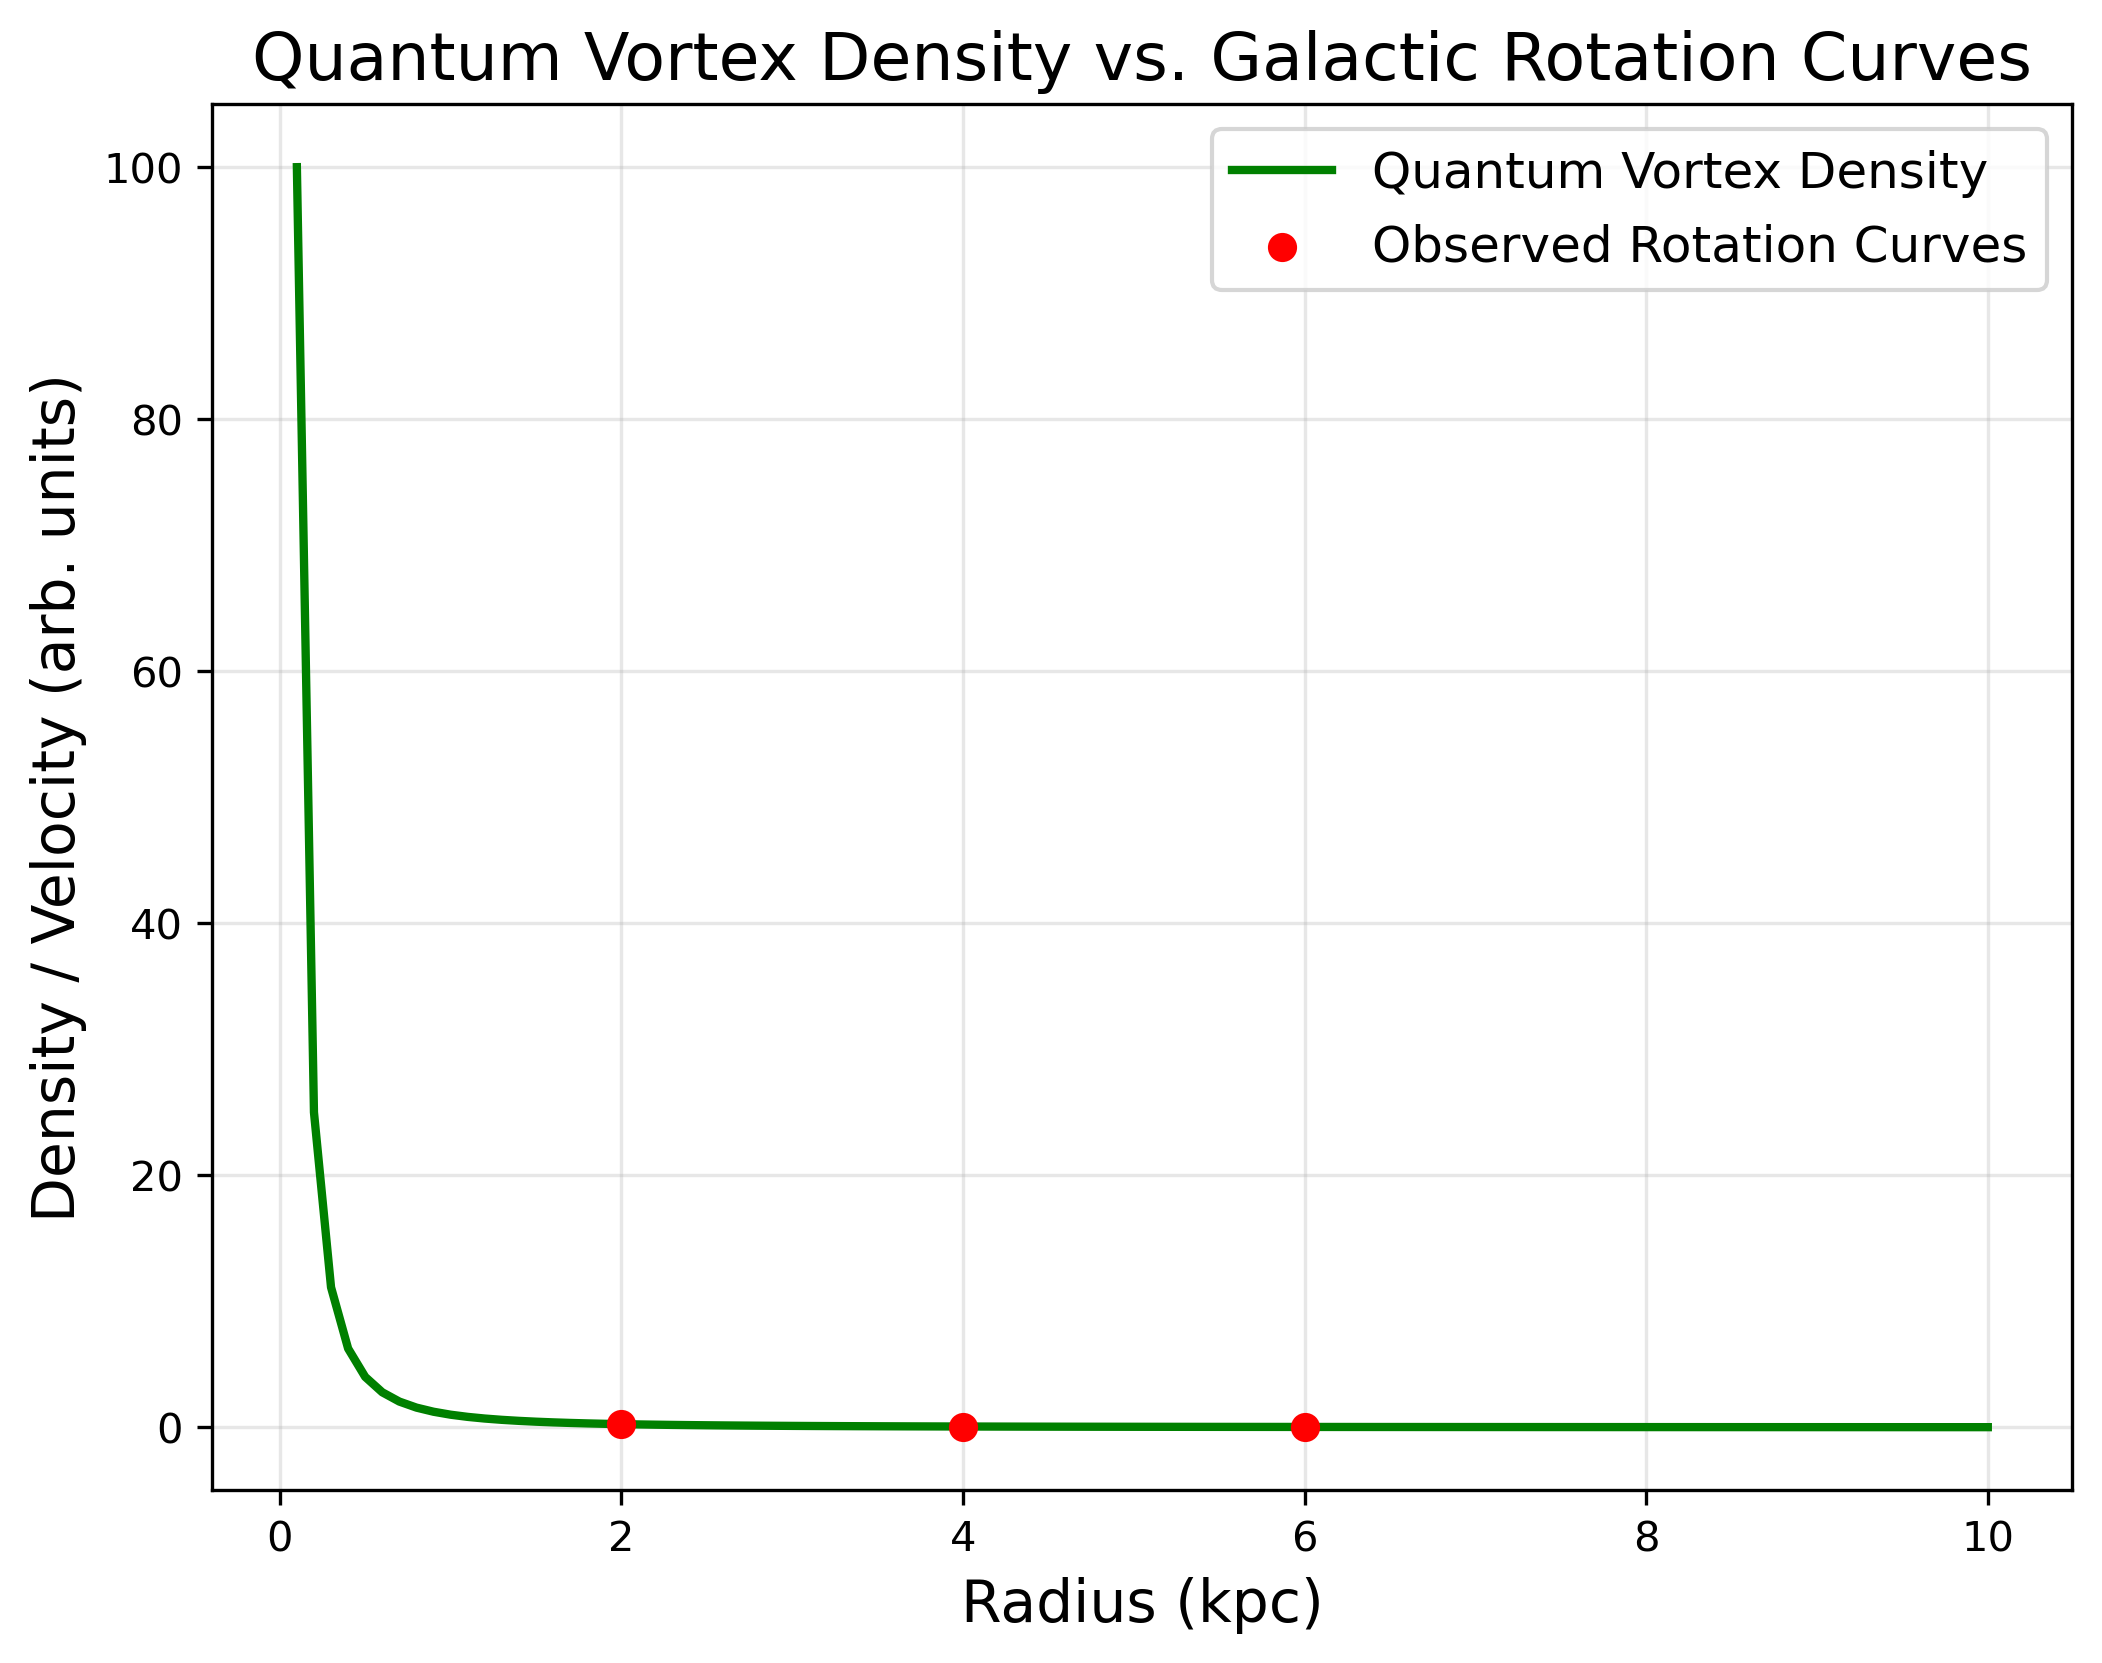
\includegraphics[width=0.8\textwidth]{dm_vortices.png}
\caption{Quantum vortex density vs. galactic rotation curves. Generated using Python.}
\label{fig:dm_vortices}
\end{figure}

\section{Axion-GRB Predictions}
Figure~\ref{fig:axion_fermi} shows the predicted 21 TeV axion-GRB flux compared to Fermi-LAT constraints. Future experiments could test this prediction.

% Place the figure here using [H]
\begin{figure}[H]
\centering
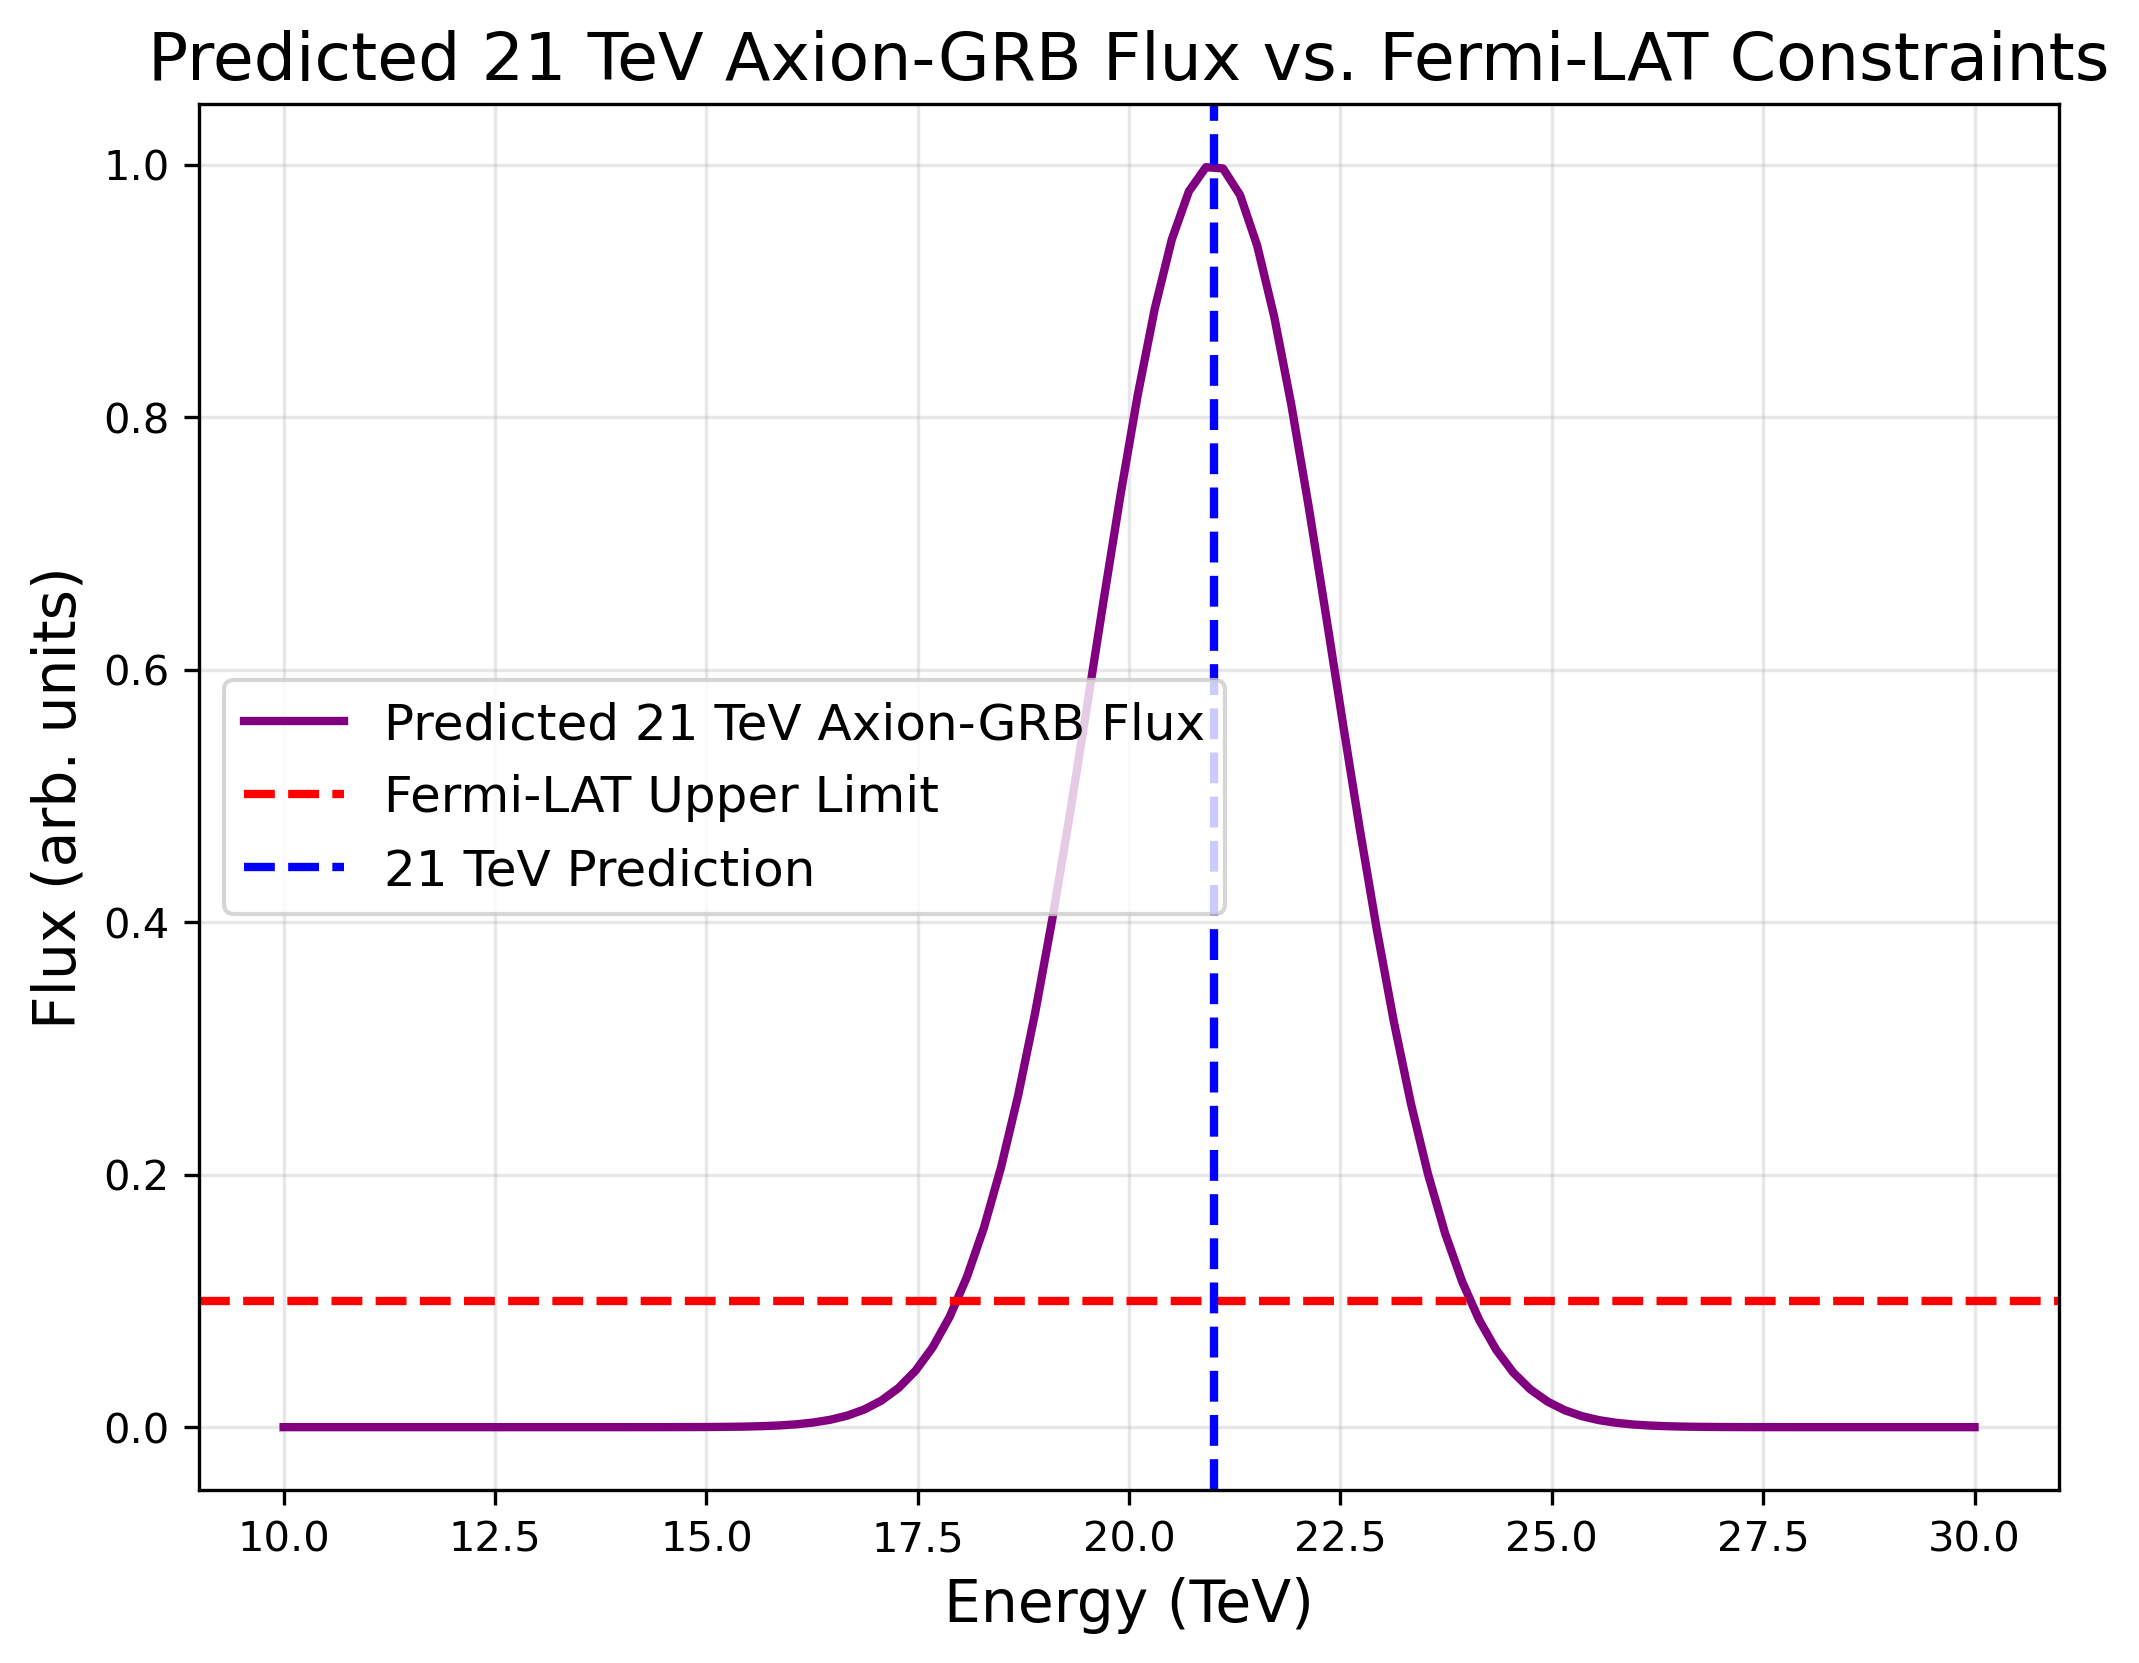
\includegraphics[width=0.8\textwidth]{axion_fermi.png}
\caption{Predicted 21 TeV axion-GRB flux vs. Fermi-LAT constraints. Generated using Python.}
\label{fig:axion_fermi}
\end{figure}

\end{document}
